\documentclass[a4paper]{article}

\usepackage{graphicx} % Required for inserting images
\usepackage[utf8]{inputenc}
\usepackage[T1]{fontenc}
\usepackage{textcomp}
\usepackage[italian]{babel}
\usepackage{amsmath, amssymb}
\usepackage{siunitx}
\usepackage{caption}
\usepackage{graphicx}
\usepackage{subcaption}
\usepackage{booktabs} % Opzionale, per tabelle più belle se vuoi (\toprule, \midrule, \bottomrule)
\usepackage{ragged2e} % Per \Centering nelle minipage
\usepackage{float} % Per [htbp]
\usepackage{fullwidth}
%\usepackage{darkmode} % Disabilitato come nell'originale
%\enabledarkmode
\usepackage[margin=2cm]{geometry}

\title{Spettrometro}
\author{Alessio Ramirez, Michele Rota, Sofia Zocchi}
\date{May 2025}

\begin{document}

\maketitle

\section{Misura con il reticolo}

\subsection{Caratterizzazione del reticolo}
\subsubsection{Obiettivo}
Determinare il passo del reticolo utilizzato a partire dall'osservazione della figura di interferenza da esso prodotta

\subsubsection{Metodo}
Innanzitutto abbiamo montato il reticolo da $300 \frac{righe}{mm}$ tra collimatore e telescopio e ne abbiamo regolato la perpendicolarità al fascio di luce. Per garantire ciò abbiamo valutato la simmetria della figura di interferenza rispetto al massimo centrale: gli angoli destro e sinistro a cui è posizionato un massimo dello stesso ordine devono risultare identici (entro l'errore di misura). Fissato come riferimento l'angolo centrale $\theta_0 \neq 0$ abbiamo verificato $|\theta_0 -\theta_{dx}|=|\theta_0 -\theta_{sx}|$, dove $\theta_{dx}$ e $\theta_{sx}$ indicano la posizione angolare del secondo doppietto giallo indicata dal goniometro. Abbiamo quindi proceduto all'identificazione del passo del reticolo $d$. E' stata utilizzata la relazione:
\begin{align}
 d\sin(\theta) = n\lambda
\label{eq:massimi reticolo}
\end{align}
la quale descrive la posizione dei massimi di interferenza da reticolo. 
Per minimizzare l'errore $\delta_{\theta}$ sulla posizione del massimo abbiamo misurato gli angoli destro e sinistro e ne abbiamo considerato poi la differenza $\theta = \frac{\theta_{dx}-\theta_{sx}}{2}$, riducendo così l'errore di un fattore $\sqrt{2}$ rispetto a considerare la media della misurazione assoluta di $\theta_{dx}$ e $\theta_{sx}$. 

\subsubsection{Dati}
Il valore di $\theta$ ottenuto è riportato in tabella \ref{tab:angoli_d}. L'errore su $\theta$ segue dalla propagazione degli errori:
\begin{align}
\delta_{theta} = \frac{1}{2}\sqrt{\delta_{theta_{dx}}^2+\delta_{theta_{sx}}^2}
\label{eq:err_angolo}
\end{align}
In particolare $\delta_{theta_{dx}} =\delta_{theta_{sx}}= 0.25^\circ$, corrispondente alla sensibilità del goniometro.
Dal momento che l'errore non dipende dalla riga spettrale osservata abbiamo scelto di studiare la posizione del secondo doppietto del sodio, e non del primo, in modo tale che l'errore relativo sul valore di $\theta$ fosse minore (essendo $\theta_1 < \theta_2$).

\begin{table}[htbp]
\centering
\begin{tabular}{|l|c|}
\hline
$\theta_{dx} [^\circ]$ & 105.25 ± 0.25 \\\hline
$\theta_{sx} [^\circ]$ & 64.25 ± 0.25 \\\hline
$\theta [^\circ]$ & 20.50 ± 0.17  \\\hline
\end{tabular}
\caption{Posizione angolare massimi di interferenza reticolo 300 righe/mm}
\label{tab:angoli_d}
\end{table}

\subsubsection{Analisi dati}
Dalla relazione \ref{eq:massimi reticolo} e dalla propagazione degli errori segue:
\begin{align}
    d = \frac{n\lambda}{\sin(\theta)}  \qquad & \text{e} \qquad \delta_d = \frac{\delta_{\theta}\cos(\theta)n\lambda}{\sin(\theta)^2}
\label{eq:passo_reticolo}
\end{align}
dove $n=2$ e $\lambda=588.995 nm$ (come riportato sul sito del NIST), considerato privo di errore.
Si è così ricavato il passo del reticolo $d=(3.36 \pm0.02)\mu m$. Tale misura è stata confrontata mediante z-test con il passo atteso $d_{att}=3.33 \mu m$, ricavato dal fatto che si è utilizzato un reticolo con $300 \frac{righe}{mm}$. 
Tale confronto e il suo risultato sono visibili in tabella \ref{tab:passo_reticolo+compatibilità}.

\begin{table}[htbp]
\centering
\begin{tabular}{|l|c|}
\hline
$d[\mu m]$ & 3.36 ± 0.05 \\\hline
$d_{att} [\mu m]$ & 3.33 \\\hline
p-value &  0.27 \\\hline
\end{tabular}
\caption{Test compatibilità passo reticolare}
\label{tab:passo_reticolo+compatibilità}
\end{table}

\subsubsection{Conclusione}
Come è possibile osservare dall'esito favorevole del test di compatibilità è presente accordo tra $d$ e $d_{att}$. 

\subsection{Studio spettro di emissione del sodio}
\subsection{Obiettivo}
Ricavato il passo reticolare a partire dall'osservazione del secondo doppietto giallo del sodio, stimare le lunghezze d'onda delle altre righe.

\subsubsection{Metodo}
Una volta montato il reticolo da $300 \frac{righe}{mm}$ e assicurata la sua perpendicolarità al fascio luminoso, abbiamo misurato l'angolo $\theta$ corrispondente alla posizione di alcune righe del sodio. Anche in questo caso abbiamo ricavato la posizione angolare dei massimi osservando entrambe le righe di ciascun doppietto, con $\theta = \frac{\theta_{dx}-\theta_{sx}}{2}$. A partire dalla relazione \ref{eq:massimi reticolo} e dalla formula generale della propagazione degli errori si è poi ricavato:
\begin{align}
    \lambda = \frac{d\sin(\theta)}{n}  \qquad & \text{e} \qquad \delta_{\lambda} = \sqrt{(\frac{\delta_{d}\sin(\theta)}{n})^2 + (\frac{\delta_{\theta}\cos(\theta)d}{n})^2}
\label{eq:lambda_sodio}
\end{align}
dove $n$ indica l'ordine del massimo osservato e $d=(3.36\pm 0.05)\mu m$ è il passo del reticolo precedentemente ricavato.
Le lunghezze d'onda osservate sono state poi confrontate sia con quelle tabulate sul sito del NIST che in parte tra di loro, dal momento che abbiamo scelto di determinare $\lambda$ per righe dello stesso colore ma appartenenti ad ordini differenti. Abbiamo infatti considerato la riga gialla del primo ordine la riga verde del primo e del secondo ordine.

\subsubsection{Dati}
Riportiamo nella tabella \ref{tab:angoli.sodio} gli angoli $\theta$ misurati. L'errore angolare proviene da $\delta_{theta}=\sqrt{\delta_{theta_{dx}}^2+\delta_{theta_{sx}}^2}$ con 
$\delta_{theta_{dx}} =\delta_{theta_{sx}}= 0.25^\circ$, sensibilità del goniometro.

\begin{table}[htbp]
\centering
\begin{tabular}{|l|c|c|c|}
\hline
 & riga gialla n=1 & riga verde n=1 & riga verde n=2 \\\hline
$\theta_{dx} [^\circ] $ & 94.5 ± 0.25 & 94 ± 0.25 & 104.25 ± 0.25  \\\hline
$\theta_{sx} [^\circ]$ &74.50 ± 0.25 & 74.75 ± 0.25 & 65.00 ± 0.25 \\\hline
$\theta [^\circ]$ &  10.00 ± 0.35 & 9.63 ± 0.35 & 19.63 ± 0.35 \\\hline
\end{tabular}
\caption{Posizione angolari righe emissione sodio}
\label{tab:angoli.sodio}
\end{table}

\subsubsection{Analisi dati}
Procedendo come prima descritto abbiamo ricavato le lunghezze d'onda corrispondenti alle righe del sodio. Esse sono raccolte in tabella \ref{tab:lunghezza_d'onda.sodio}. Quanto misurato è stato poi confrontato con le lunghezze d'onda tabulate mediante z-test, con $z=\frac{|\lambda-\lambda_{att}|}{\delta_{\lambda}}$

\begin{table}[htbp]
\centering
\begin{tabular}{|l|c|c|c|c|}
\hline
 & riga gialla n=1 & riga verde n=1 & riga verde n=2  \\\hline
$\lambda [nm] $ & 583 ± 20 & 562 ± 20 & 565 ± 10 \\\hline
$\lambda_{att} [nm]$ & 589 & 568 & 568 \\\hline
p-value & 0.38 & 0.38 & 0.38 \\\hline
\end{tabular}
\caption{Righe d'emissione sodio}
\label{tab:lunghezza_d'onda.sodio}
\end{table}

Si è valutata poi anche compatibilità tra le due lunghezze d'onda ricavate sperimentalmente per la riga d'emissione verde. Esse distano $0.1\sigma$ e possono considerarsi quindi in accordo.

\subsubsection{Conclusione}
Seppur lo spettro di emissione del sodio sia stato valutato solo parzialmente, possiamo attribuire allo studio mediante reticolo di diffrazione esito positivo, infatti tutti i test di compatibilità effettuati mettono accordo tra $\lambda$ ricavata sperimentalmente e $\lambda_{att}$. Possiamo poi osservare come l'errore sulla lunghezza d'onda non dipenda da $\lambda$ ma sia inversamente proporzionale all'ordine del massimo ($\delta_{\lambda} \propto \frac{1}{n}$), diminuisce quindi all'aumentare di $n$. 



\subsection{Confronto tra reticoli di differente passo}

\subsubsection{Obiettivo}
Confrontare le caratteristiche di reticoli di diffrazione aventi un passo differente (reticoli a $600 \frac{righe}{mm}$ e $1200 \frac{righe}{mm}$. Determinare sperimentalmente il loro passo e valutarne potere dispersivo e risolutivo.

\subsubsection{Metodo}
Come nelle esperienze precedenti si è proceduto dall'osservazione delle figure di interferenza. Tali figure sono state osservate dopo aver montato reticoli differenti tra telescopio e collimatore e averne realizzato la calibrazione. Per la determinazione del passo $d$ dei reticoli di diffrazione si è proceduto come in precedenza. Vogliamo però sottolineare come nell'utilizzo del reticolo da $1200 \frac{righe}{mm}$ abbiamo potuto prendere in considerazione soltanto l'angolo $\theta$ corrispondente alla posizione angolare del primo massimo di interferenza, dal momento che i massimi del secondo ordine risultavano esterni al nostro campo visivo. Tale fenomeno è da attribuirsi al diverso potere risolutivo $R$ dei vari reticoli. Esso quantifica la capacità di osservare due lunghezze d'onda differenti in corrispondenza di un massimo di ordine $n$, ed è definito $R=nN$, dove $N$ indica il numero di fenditure del reticolo illuminate. All'aumentare del numero di righe al $mm$ $N$ aumenta e di conseguenza si ha un migliore potere risolutivo, il quale si traduce nell'osservazione di righe spettrali più distanziate tra di loro e di fatto non si ha spazio per la visualizzazione dei massimi di ordine successivo, troppo esterni.
Inoltre dall'utilizzo di reticoli aventi passo differente abbiamo potuto valutarne anche il potere dispersivo $D=\frac{n}{d\cos{\theta_n}}$, dove $n$ indica l'ordine del massimo, $\theta_n$ la sua posizione angolare e $d$ il passo del reticolo. Ad un maggiore numero di righe al $mm$, cioè a un minore passo $d$, corrisponde un maggiore potere dispersivo, ossia le righe osservate hanno larghezza maggiore. A ragion di ciò per i reticoli a $600 \frac{righe}{mm}$ e $1200 \frac{righe}{mm}$ nel misurare $\theta_{dx}$ e $\theta_{sx}$ si è considerato un errore maggiore rispetto alle attività precedenti, essendo più difficile identificare con precisione la posizione angolare delle righe.

\subsubsection{Dati}
I valori di $\theta$ ottenuti per i due reticoli sono riportati nelle tabelle \ref{tab:angoli_600} e \ref{tab:angoli_1200}. L'errore su $\theta$ segue dalla propagazione degli errori:
\begin{align}
\delta_{theta} = \sqrt{\delta_{theta_{dx}}^2+\delta_{theta_{sx}}^2}
\end{align}
con $\delta_{theta_{dx}} =\delta_{theta_{sx}}= 0.5^\circ$.

\begin{table}[htbp]
\centering
\begin{tabular}{|l|c|}
\hline
$\theta_{dx} [^\circ]$ & 127 ± 0.5 \\\hline
$\theta_{sx} [^\circ]$ & 37.5 ± 0.5 \\\hline
$\theta [^\circ]$ & 44.75 ± 0.7  \\\hline
\end{tabular}
\caption{Posizione angolare massimi di interferenza reticolo 600 righe/mm}
\label{tab:angoli_600}
\end{table}

\begin{table}[htbp]
\centering
\begin{tabular}{|l|c|}
\hline
$\theta_{dx} [^\circ]$ & 127 ± 0.5 \\\hline
$\theta_{sx} [^\circ]$ & 37.5 ± 0.5 \\\hline
$\theta [^\circ]$ & 44.75 ± 0.70  \\\hline
\end{tabular}
\caption{Posizione angolare massimi di interferenza reticolo 1200 righe/mm}
\label{tab:angoli_1200}
\end{table}

\subsubsection{Analisi dati}
Così come nel caso precedente per la determinazione del passo $d$ dei reticoli sono state applicate le relazione \ref{eq:massimi reticolo} e \ref{eq:passo_reticolo}. Il valore di $\lambda=588.995 nm$ è stato considerato senza errore. Si ha poi $n=2$ per il reticolo da $600 \frac{righe}{mm}$ (osservazione dei massimi del secondo ordine) e $n=1$ per il reticolo da $1200 \frac{righe}{mm}$ (osservazione limitata ai massimi del primo ordine). I valori di $d$ ricavati sperimentalmente sono poi stati ricavati con quanto atteso. Tale confronto è stato attuato mediante z-test con $z = \frac{|d-d_{att}|}{\delta_d}$ e i suoi risultati sono raccolti in tabella \ref{tab:passi+test_compatibilità}.

\begin{table}[htbp]
\centering
\begin{tabular}{|l|c|c|}
\hline
 & $600 \frac{righe}{mm}$ & $1200 \frac{righe}{mm}$ \\\hline
$d$ & 1.673 ± 0.021 $[\mu m]$ & 836.623 ± 10.311 $[nm]$\\\hline
$d_{att} $ & 1.667 $[\mu m]$ & 833.333 $[nm]$\\\hline
p-value &  0.39 & 0.37 \\\hline
\end{tabular}
\caption{Studio passi reticolari}
\label{tab:passi+test_compatibilità}
\end{table}

\subsubsection{Conclusione}
Come per la prima parte di misurazioni effettuate con il reticolo possiamo considerare quanto ricavato come coerente con il risultato atteso; sia per quanto riguarda il valore del passo reticolare (z-test mostra accordo tra $d$ e $d_{att}$), sia per l'osservazione degli effetti dovuti a poteri risolutivi e dispersivi differenti.




\section{Misure con il prisma}
\subsubsection{Obiettivo}
Caratterizzare un prisma a dispersione: valutarne le caratteristiche geometriche e determinare i parametri della legge di Cauchy che ne descrive l'indice di rifrazione.

\subsubsection{Metodo}
Una volta completata la messa a fuoco dello spettrometro abbiamo posizionato il prisma a dispersione sulla piattaforma posta tra telescopio e collimatore. Nonostante la regolazione della piattaforma, quest'ultima non era perfettamente complanare con l'asse congiungente collimatore e oculare; di conseguenza il posizionamento del prisma non è avvenuto centralmente rispetto alla piattaforma, per poter fare in modo che i raggi luminosi rifratti fossero individuabili dal telescopio.
\newline
\newline
\textbf{Angolo al vertice} \newline
Per determinare l'angolo al vertice $\alpha$ si è sfruttato il potere riflessivo delle due facce lucide del prisma. Abbiamo dapprima ruotato il telescopio posizionandolo ad un angolo $\theta_i$ tale per cui risultava visibile il raggio riflesso proveniente dalla prima faccia lucida del prisma. Abbiamo poi ruotato la piattaforma (quindi il prisma posto su di essa) fino ad individuare nuovamente con il telescopio il raggio riflesso dalla seconda faccia lucida del prisma, visibile dopo una rotazione di un angolo $\beta$. L'angolo al vertice risulta quindi:
\begin{align}
    \alpha = \frac{\theta_i -\beta}{2}
\label{eq:angolo al vertice}
\end{align}
\textbf{Angolo di minima deviazione}\newline
Per la determinazione dell'angolo di minima deviazione è stata utilizzata una lampada al mercurio, in modo da poter considerare note a priori (e quindi prive di errore) le lunghezze d'onda delle singole righe d'emissione, ricavate dal sito del NIST.
Sono state prese in considerazione 5 diverse righe spettrali. La prima riga corrisponde al doppietto giallo più intenso del mercurio, le cui righe sono state considerate come sovrapposte, in quanto difficili da distinguere, con lunghezza d'onda media di quelle indicate sul sito del NIST.
L'angolo di minima deviazione corrisponde alla posizione angolare tale per cui la deviazione interna dovuta alla rifrazione del raggio incidente è minimizzata. Tale angolo dipende dal potere rifrattivo del prisma (quindi dal suo indice di rifrazione $n$), a sua volta dipendente dalla lunghezza d'onda della radiazione; di conseguenza variabile a seconda della riga spettrale osservata. In particolare si ha:
\begin{align}
    \sin(\frac{\theta_m + \alpha}{2}) = n\sin(\frac{\alpha}{2})
\label{eq:angolo min deviazione}
\end{align}
Quindi per determinare $n$ indice di rifrazione si è utilizzata la relazione:
\begin{align}
    n= \frac{\sin(\frac{\theta_m + \alpha}{2})}{\sin(\frac{\alpha}{2})}
\label{eq:indice di rifrazione}
\end{align}
La misura di $\theta_m$ è stata effettuata determinando la posizione del prisma per cui si aveva un'inversione del moto della riga spettrale rispetto alla rotazione del prisma. Più precisamente scelta una determinata riga spettrale l'abbiamo seguita con il telescopio, ruotandolo simultaneamente alla piattaforma fino a quando la riga non tornava indietro e si misurava l'angolo rispetto alla direzione del raggio in-deflesso (cioè alla congiungente telescopio-collimatore). L'angolo di minima deviazione è quindi determinato da: 
\begin{align}
    \theta_m = \theta_0-\theta_R
\label{eq:posizione zero}
\end{align}
dove $\theta_0$ indica la posizione angolare dello zero e $\theta_R$ la posizione angolare del telescopio necessaria a osservare l'angolo di minima deviazione.
\newline\\
\textbf{Legge di Cauchy} \newline
Determinato l'angolo di minima deviazione corrispondente a ogni lunghezza d'onda abbiamo proceduto allo studio della relazione tra $\lambda$ e $n$, descritta dalla legge di Cauchy:
\begin{align}
    n(\lambda) = A + \frac{B}{\lambda^2} + ...
\label{eq:Cauchy}
\end{align}
al fine di determinare i parametri $A$ e $B$.

\subsubsection{Dati}
Per quanto riguarda l'angolo al vertice abbiamo misurato $\theta_i = (145.50\pm0.25)^\circ$ e $\beta=(19.0\pm0.25)^\circ$. \footnote{Tutti gli angoli sono stati misurati mediante l'utilizzo del goniometro posto sulla piattaforma. Lo zero coincide quindi con il valore $0$ del goniometro.} L'errore è stato valutato uguale per tutti gli angoli, $\delta_{\theta}=0.25^\circ$, corrispondente alla sensibilità del goniometro, ne consegue che per propagazione degli errori l'errore su $\alpha$ si riduce di un fattore $\sqrt{2}$. Abbiamo scelto di considerare come errore la sensibilità dal momento che le misure angolari non sono risultate affette da errore casuale. Per confermare ciò abbiamo provato a ripetere una misura di $\theta_m$ e abbiamo riottenuto lo stesso valore, entro la sensibilità di misura. Si ha quindi $\alpha = (61.8 \pm 0.2)^\circ$. 
Quanto misurato e utilizzato per ricavare $\theta_m$ e $n(\lambda)$ per ciascuna lunghezza d'onda $\lambda_i$ secondo le relazioni \ref{eq:posizione zero} e \ref{eq:angolo min deviazione} si trova in tabella \ref{tab:indice di rifrazione e angoli}. Gli errori sull'indice di rifrazione $\delta_n$ sono ricavati applicando la formula generale della propagazione degli errori alla relazione \ref{eq:indice di rifrazione}, da cui si ottiene:
\begin{align}
    \delta_n = \sqrt{(\frac{\cos(\frac{\alpha+\theta_m}{2})\sin(\frac{\alpha}{2})-\cos(\frac{\alpha}{2})\sin(\frac{\alpha+\theta_m}{2})}{2\sin^2(\frac{\alpha}{2})}\delta_{\alpha})^2+(\frac{\delta_{\theta_m}\cos(\frac{\alpha+\theta_m}{2})}{2\sin(\frac{\alpha}{2})})^2}
\end{align}

\begin{table}[htbp]
\centering
\begin{tabular}{|l|ccccc|}
\hline
$\lambda [nm]$ & 578.0134 & 546.9598 & 435.8328 & 434.7500 & 404.6563 \\\hline
$\theta_R [^\circ]$ & 48.5 ± 0.3 & 47.5 ± 0.3 & 47.0 ± 0.3 & 47.5 ± 0.3 & 47.5 ± 0.3 \\\hline
$\theta_0 [^\circ]$ & 97.0 ± 0.3 & 95.5 ± 0.3 & 96.5 ± 0.3 & 98.0 ± 0.3 & 99.0 ± 0.3 \\\hline
$\theta_m [^\circ]$ & 48.5 ± 0.4 & 48.0 ± 0.4 & 49.5 ± 0.4 & 50.5 ± 0.4 & 51.5 ± 0.4 \\\hline
n & 1.599 ± 0.006 & 1.594 ± 0.006 & 1.608 ± 0.006 & 1.618 ± 0.006 & 1.627 ± 0.006 \\\hline
\end{tabular}
\caption{Angolo di minima deviazione e indice di rifrazione per ciascuna riga}
\label{tab:indice di rifrazione e angoli}
\end{table}

\subsubsection{Analisi dati}

\begin{figure}[htbp]
	\centering
	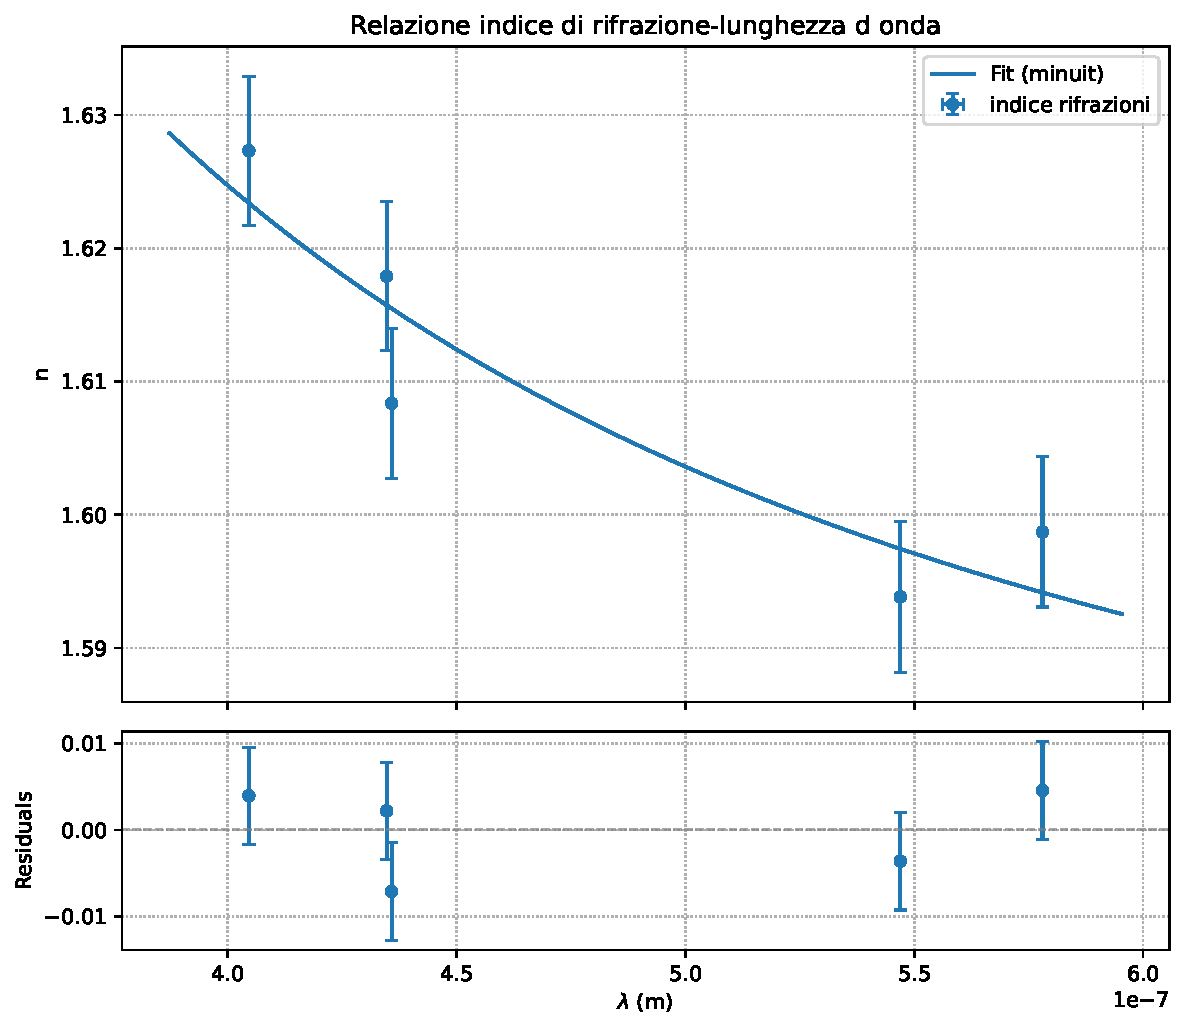
\includegraphics[width=0.5\textwidth]{grafici/cauchy.pdf}
	\caption{Andamento fit legge di Cauchy}
	\label{fig:grafico cauchy}
\end{figure}

Per lo studio dell'andamento $n(\lambda)$ abbiamo interpolato i dati presenti in \ref{tab:indice di rifrazione e angoli} con la relazione di Cauchy \ref{eq:Cauchy}. La miglior stima di $A$ e $B$ figura in tabella \ref{tab:fit cauchy}, affiancata dai risultati del test del chi quadro applicato al fit.
Il medesimo fit è rappresentato nel grafico \ref{fig:grafico cauchy}.

\begin{table}[htbp]
\centering
\begin{tabular}{|l|ccccc|}
\hline
Fit & A & B & $\chi^2$ & DoF & $\chi^2/\nu$ \\\hline\hline
Risultati & 1.5660 ± 0.0099 & 9.4 ± 2.1 f & 3.31 & 3 & 1.1 \\\hline
\end{tabular}
\caption{Risultati fit legge di Cauchy}
\label{tab:fit cauchy}
\end{table}

\subsubsection{Conclusione}
%commentare perchè si arresta sviluppo al secondo ordine (b piccolo), come si è scelto quante righe misurare, immagine del fit
\subsubsection{Conclusione}
L'esperimento ha permesso di caratterizzare con successo le proprietà del prisma. Misurando l'angolo di minima deviazione per cinque righe spettrali del mercurio, come riportato in Tabella \ref{tab:indice di rifrazione e angoli}, è stato possibile determinare la relazione tra l'indice di rifrazione e la lunghezza d'onda.
I dati sono stati interpolati usando la legge di Cauchy, arrestando lo sviluppo al termine in $1/\lambda^2$. Questa scelta è giustificata sia dal piccolo valore del parametro $B$ ottenuto (Tabella \ref{tab:fit cauchy}), che suggerisce una rapida convergenza della serie, sia dall'esito del test del chi-quadro. Il valore di $\chi^2/\nu = 1.1$ indica un'eccellente compatibilità tra il modello e i dati sperimentali, rendendo superfluo l'inserimento di ulteriori parametri, inoltre l'utilizzo di "sole" 5 righe spettrali è giustificato dal fatto che per altre righe avremmo dovuto utilizzare errori almeno il doppio più grandi.
In definitiva, la procedura si è dimostrata valida e ha portato a una stima precisa dei parametri di Cauchy del prisma, confermando la validità di tale legge per descrivere la dispersione nel materiale analizzato.


\end{document}

